% Options for packages loaded elsewhere
\PassOptionsToPackage{unicode}{hyperref}
\PassOptionsToPackage{hyphens}{url}
%
\documentclass[
]{article}
\usepackage{lmodern}
\usepackage{amssymb,amsmath}
\usepackage{ifxetex,ifluatex}
\ifnum 0\ifxetex 1\fi\ifluatex 1\fi=0 % if pdftex
  \usepackage[T1]{fontenc}
  \usepackage[utf8]{inputenc}
  \usepackage{textcomp} % provide euro and other symbols
\else % if luatex or xetex
  \usepackage{unicode-math}
  \defaultfontfeatures{Scale=MatchLowercase}
  \defaultfontfeatures[\rmfamily]{Ligatures=TeX,Scale=1}
\fi
% Use upquote if available, for straight quotes in verbatim environments
\IfFileExists{upquote.sty}{\usepackage{upquote}}{}
\IfFileExists{microtype.sty}{% use microtype if available
  \usepackage[]{microtype}
  \UseMicrotypeSet[protrusion]{basicmath} % disable protrusion for tt fonts
}{}
\makeatletter
\@ifundefined{KOMAClassName}{% if non-KOMA class
  \IfFileExists{parskip.sty}{%
    \usepackage{parskip}
  }{% else
    \setlength{\parindent}{0pt}
    \setlength{\parskip}{6pt plus 2pt minus 1pt}}
}{% if KOMA class
  \KOMAoptions{parskip=half}}
\makeatother
\usepackage{xcolor}
\IfFileExists{xurl.sty}{\usepackage{xurl}}{} % add URL line breaks if available
\IfFileExists{bookmark.sty}{\usepackage{bookmark}}{\usepackage{hyperref}}
\hypersetup{
  pdftitle={Microsimulation Sick-Sicker model with time dependency},
  pdfauthor={The DARTH workgroup},
  hidelinks,
  pdfcreator={LaTeX via pandoc}}
\urlstyle{same} % disable monospaced font for URLs
\usepackage[margin=1in]{geometry}
\usepackage{color}
\usepackage{fancyvrb}
\newcommand{\VerbBar}{|}
\newcommand{\VERB}{\Verb[commandchars=\\\{\}]}
\DefineVerbatimEnvironment{Highlighting}{Verbatim}{commandchars=\\\{\}}
% Add ',fontsize=\small' for more characters per line
\usepackage{framed}
\definecolor{shadecolor}{RGB}{248,248,248}
\newenvironment{Shaded}{\begin{snugshade}}{\end{snugshade}}
\newcommand{\AlertTok}[1]{\textcolor[rgb]{0.94,0.16,0.16}{#1}}
\newcommand{\AnnotationTok}[1]{\textcolor[rgb]{0.56,0.35,0.01}{\textbf{\textit{#1}}}}
\newcommand{\AttributeTok}[1]{\textcolor[rgb]{0.77,0.63,0.00}{#1}}
\newcommand{\BaseNTok}[1]{\textcolor[rgb]{0.00,0.00,0.81}{#1}}
\newcommand{\BuiltInTok}[1]{#1}
\newcommand{\CharTok}[1]{\textcolor[rgb]{0.31,0.60,0.02}{#1}}
\newcommand{\CommentTok}[1]{\textcolor[rgb]{0.56,0.35,0.01}{\textit{#1}}}
\newcommand{\CommentVarTok}[1]{\textcolor[rgb]{0.56,0.35,0.01}{\textbf{\textit{#1}}}}
\newcommand{\ConstantTok}[1]{\textcolor[rgb]{0.00,0.00,0.00}{#1}}
\newcommand{\ControlFlowTok}[1]{\textcolor[rgb]{0.13,0.29,0.53}{\textbf{#1}}}
\newcommand{\DataTypeTok}[1]{\textcolor[rgb]{0.13,0.29,0.53}{#1}}
\newcommand{\DecValTok}[1]{\textcolor[rgb]{0.00,0.00,0.81}{#1}}
\newcommand{\DocumentationTok}[1]{\textcolor[rgb]{0.56,0.35,0.01}{\textbf{\textit{#1}}}}
\newcommand{\ErrorTok}[1]{\textcolor[rgb]{0.64,0.00,0.00}{\textbf{#1}}}
\newcommand{\ExtensionTok}[1]{#1}
\newcommand{\FloatTok}[1]{\textcolor[rgb]{0.00,0.00,0.81}{#1}}
\newcommand{\FunctionTok}[1]{\textcolor[rgb]{0.00,0.00,0.00}{#1}}
\newcommand{\ImportTok}[1]{#1}
\newcommand{\InformationTok}[1]{\textcolor[rgb]{0.56,0.35,0.01}{\textbf{\textit{#1}}}}
\newcommand{\KeywordTok}[1]{\textcolor[rgb]{0.13,0.29,0.53}{\textbf{#1}}}
\newcommand{\NormalTok}[1]{#1}
\newcommand{\OperatorTok}[1]{\textcolor[rgb]{0.81,0.36,0.00}{\textbf{#1}}}
\newcommand{\OtherTok}[1]{\textcolor[rgb]{0.56,0.35,0.01}{#1}}
\newcommand{\PreprocessorTok}[1]{\textcolor[rgb]{0.56,0.35,0.01}{\textit{#1}}}
\newcommand{\RegionMarkerTok}[1]{#1}
\newcommand{\SpecialCharTok}[1]{\textcolor[rgb]{0.00,0.00,0.00}{#1}}
\newcommand{\SpecialStringTok}[1]{\textcolor[rgb]{0.31,0.60,0.02}{#1}}
\newcommand{\StringTok}[1]{\textcolor[rgb]{0.31,0.60,0.02}{#1}}
\newcommand{\VariableTok}[1]{\textcolor[rgb]{0.00,0.00,0.00}{#1}}
\newcommand{\VerbatimStringTok}[1]{\textcolor[rgb]{0.31,0.60,0.02}{#1}}
\newcommand{\WarningTok}[1]{\textcolor[rgb]{0.56,0.35,0.01}{\textbf{\textit{#1}}}}
\usepackage{graphicx,grffile}
\makeatletter
\def\maxwidth{\ifdim\Gin@nat@width>\linewidth\linewidth\else\Gin@nat@width\fi}
\def\maxheight{\ifdim\Gin@nat@height>\textheight\textheight\else\Gin@nat@height\fi}
\makeatother
% Scale images if necessary, so that they will not overflow the page
% margins by default, and it is still possible to overwrite the defaults
% using explicit options in \includegraphics[width, height, ...]{}
\setkeys{Gin}{width=\maxwidth,height=\maxheight,keepaspectratio}
% Set default figure placement to htbp
\makeatletter
\def\fps@figure{htbp}
\makeatother
\setlength{\emergencystretch}{3em} % prevent overfull lines
\providecommand{\tightlist}{%
  \setlength{\itemsep}{0pt}\setlength{\parskip}{0pt}}
\setcounter{secnumdepth}{-\maxdimen} % remove section numbering

\title{Microsimulation Sick-Sicker model with time dependency}
\usepackage{etoolbox}
\makeatletter
\providecommand{\subtitle}[1]{% add subtitle to \maketitle
  \apptocmd{\@title}{\par {\large #1 \par}}{}{}
}
\makeatother
\subtitle{Includes individual characteristics: age, age dependent mortality
probabilities, individual treatment effect modifyer, state-residency for
the sick (S1) state, increasing change of death in the first 6 year of
sickness (tunnel)}
\author{The DARTH workgroup}
\date{}

\begin{document}
\maketitle

Developed by the Decision Analysis in R for Technologies in Health
(DARTH) workgroup:

Fernando Alarid-Escudero, PhD (1)

Eva A. Enns, MS, PhD (2)

M.G. Myriam Hunink, MD, PhD (3,4)

Hawre J. Jalal, MD, PhD (5)

Eline M. Krijkamp, MSc (3)

Petros Pechlivanoglou, PhD (6)

Alan Yang, MSc (7)

In collaboration of:

\begin{enumerate}
\def\labelenumi{\arabic{enumi}.}
\tightlist
\item
  Drug Policy Program, Center for Research and Teaching in Economics
  (CIDE) - CONACyT, Aguascalientes, Mexico
\item
  University of Minnesota School of Public Health, Minneapolis, MN, USA
\item
  Erasmus MC, Rotterdam, The Netherlands
\item
  Harvard T.H. Chan School of Public Health, Boston, USA
\item
  University of Pittsburgh Graduate School of Public Health, Pittsburgh,
  PA, USA
\item
  University of Toronto, Toronto ON, Canada
\item
  The Hospital for Sick Children, Toronto ON, Canada
\end{enumerate}

Please cite our publications when using this code:

\begin{itemize}
\item
  Jalal H, Pechlivanoglou P, Krijkamp E, Alarid-Escudero F, Enns E,
  Hunink MG. An Overview of R in Health Decision Sciences. Med Decis
  Making. 2017; 37(3): 735-746.
  \url{https://journals.sagepub.com/doi/abs/10.1177/0272989X16686559}
\item
  Krijkamp EM, Alarid-Escudero F, Enns EA, Jalal HJ, Hunink MGM,
  Pechlivanoglou P. Microsimulation modeling for health decision
  sciences using R: A tutorial. Med Decis Making. 2018;38(3):400--22.
  \url{https://journals.sagepub.com/doi/abs/10.1177/0272989X18754513}
\item
  Krijkamp EM, Alarid-Escudero F, Enns E, Pechlivanoglou P, Hunink MM,
  Jalal H. A Multidimensional Array Representation of State-Transition
  Model Dynamics. Med Decis Making. 2020 Online first.
  \url{https://doi.org/10.1177/0272989X19893973}
\end{itemize}

Copyright 2017, THE HOSPITAL FOR SICK CHILDREN AND THE COLLABORATING
INSTITUTIONS. All rights reserved in Canada, the United States and
worldwide. Copyright, trademarks, trade names and any and all associated
intellectual property are exclusively owned by THE HOSPITAL FOR Sick
CHILDREN and the collaborating institutions. These materials may be
used, reproduced, modified, distributed and adapted with proper
attribution.

\newpage

\begin{Shaded}
\begin{Highlighting}[]
\KeywordTok{rm}\NormalTok{(}\DataTypeTok{list =} \KeywordTok{ls}\NormalTok{())      }\CommentTok{# clear memory (removes all the variables from the workspace)}
\end{Highlighting}
\end{Shaded}

\hypertarget{load-packages}{%
\section{01 Load packages}\label{load-packages}}

\begin{Shaded}
\begin{Highlighting}[]
\ControlFlowTok{if}\NormalTok{ (}\OperatorTok{!}\KeywordTok{require}\NormalTok{(}\StringTok{'pacman'}\NormalTok{)) }\KeywordTok{install.packages}\NormalTok{(}\StringTok{'pacman'}\NormalTok{); }\KeywordTok{library}\NormalTok{(pacman) }\CommentTok{# use this package to conveniently install other packages}
 \CommentTok{# load (install if required) packages from CRAN}
 \KeywordTok{p_load}\NormalTok{(}\StringTok{"here"}\NormalTok{, }\StringTok{"dplyr"}\NormalTok{, }\StringTok{"devtools"}\NormalTok{, }\StringTok{"scales"}\NormalTok{, }\StringTok{"ellipse"}\NormalTok{, }\StringTok{"ggplot2"}\NormalTok{, }\StringTok{"lazyeval"}\NormalTok{, }\StringTok{"igraph"}\NormalTok{, }\StringTok{"ggraph"}\NormalTok{, }\StringTok{"reshape2"}\NormalTok{, }\StringTok{"knitr"}\NormalTok{)                                               }
 \CommentTok{# load (install if required) packages from GitHub}
 \CommentTok{# install_github("DARTH-git/dampack", force = TRUE) Uncomment if there is a newer version}
 \KeywordTok{p_load_gh}\NormalTok{(}\StringTok{"DARTH-git/dampack"}\NormalTok{) }
\end{Highlighting}
\end{Shaded}

\hypertarget{load-functions}{%
\section{02 Load functions}\label{load-functions}}

\begin{Shaded}
\begin{Highlighting}[]
\KeywordTok{source}\NormalTok{(}\StringTok{"Functions.R"}\NormalTok{)}
\end{Highlighting}
\end{Shaded}

\hypertarget{input-model-parameters}{%
\section{03 Input model parameters}\label{input-model-parameters}}

\begin{Shaded}
\begin{Highlighting}[]
\KeywordTok{set.seed}\NormalTok{(}\DecValTok{1}\NormalTok{)  }\CommentTok{# set the seed  }

\CommentTok{# Model structure }
\NormalTok{n_t   <-}\StringTok{ }\DecValTok{30}                       \CommentTok{# time horizon, 30 cycles}
\NormalTok{n_i   <-}\StringTok{ }\DecValTok{100000}                   \CommentTok{# number of simulated individuals}
\NormalTok{v_n   <-}\StringTok{ }\KeywordTok{c}\NormalTok{(}\StringTok{"H"}\NormalTok{, }\StringTok{"S1"}\NormalTok{, }\StringTok{"S2"}\NormalTok{, }\StringTok{"D"}\NormalTok{)  }\CommentTok{# the model states names}
\NormalTok{n_states   <-}\StringTok{ }\KeywordTok{length}\NormalTok{(v_n)              }\CommentTok{# the number of health states}
\NormalTok{d_r   <-}\StringTok{ }\FloatTok{0.03}                     \CommentTok{# discount rate of 3% per cycle}
\NormalTok{v_dwe <-}\StringTok{ }\NormalTok{v_dwc <-}\StringTok{ }\DecValTok{1} \OperatorTok{/}\StringTok{ }\NormalTok{((}\DecValTok{1} \OperatorTok{+}\StringTok{ }\NormalTok{d_r) }\OperatorTok{^}\StringTok{ }\NormalTok{(}\DecValTok{0}\OperatorTok{:}\NormalTok{n_t))    }\CommentTok{# discount weight }
\NormalTok{v_names_str <-}\StringTok{ }\KeywordTok{c}\NormalTok{(}\StringTok{"no treatment"}\NormalTok{, }\StringTok{"treatment"}\NormalTok{)  }\CommentTok{# strategy names}
\NormalTok{n_str <-}\StringTok{ }\KeywordTok{length}\NormalTok{(v_names_str)      }\CommentTok{# number of strategies}

\CommentTok{### Event probabilities (per cycle)}
\CommentTok{# Annual transition probabilities}
\NormalTok{p_HS1   <-}\StringTok{ }\FloatTok{0.15}                   \CommentTok{# probability of becoming sick when healthy}
\NormalTok{p_S1H   <-}\StringTok{ }\FloatTok{0.5}                    \CommentTok{# probability of recovering to healthy when sick}
\NormalTok{p_S1S2  <-}\StringTok{ }\FloatTok{0.105}                  \CommentTok{# probability of becoming sicker when sick}

\CommentTok{# Annual probabilities of death}
\CommentTok{# load age dependent probability}
\NormalTok{p_mort   <-}\StringTok{ }\KeywordTok{read.csv}\NormalTok{(}\StringTok{"mortProb_age.csv"}\NormalTok{)}
\CommentTok{# load age distribution}
\NormalTok{dist_Age <-}\StringTok{ }\KeywordTok{read.csv}\NormalTok{(}\StringTok{"MyPopulation-AgeDistribution.csv"}\NormalTok{) }

\CommentTok{# probability to die in S1 by cycle (is increasing)}
\NormalTok{p_S1D    <-}\StringTok{ }\KeywordTok{c}\NormalTok{(}\FloatTok{0.0149}\NormalTok{, }\FloatTok{0.018}\NormalTok{, }\FloatTok{0.021}\NormalTok{, }\FloatTok{0.026}\NormalTok{, }\FloatTok{0.031}\NormalTok{, }\KeywordTok{rep}\NormalTok{(}\FloatTok{0.037}\NormalTok{, n_t }\OperatorTok{-}\StringTok{ }\DecValTok{5}\NormalTok{)) }
\NormalTok{p_S2D    <-}\StringTok{ }\FloatTok{0.048}           \CommentTok{# probability to die in S2}

\CommentTok{# Cost inputs}
\NormalTok{c_H     <-}\StringTok{ }\DecValTok{2000}             \CommentTok{# cost of one cycle in the healthy state}
\NormalTok{c_S1    <-}\StringTok{ }\DecValTok{4000}             \CommentTok{# cost of one cycle in the sick state  }
\NormalTok{c_S2    <-}\StringTok{ }\DecValTok{15000}            \CommentTok{# cost of one cycle in the sicker state}
\NormalTok{c_D     <-}\StringTok{ }\DecValTok{0}                \CommentTok{# cost of one cycle in the dead state}
\NormalTok{c_Trt   <-}\StringTok{ }\DecValTok{12000}            \CommentTok{# cost of treatment (per cycle)}

\CommentTok{# Utility inputs}
\NormalTok{u_H     <-}\StringTok{ }\DecValTok{1}                \CommentTok{# utility when healthy }
\NormalTok{u_S1    <-}\StringTok{ }\FloatTok{0.75}             \CommentTok{# utility when sick }
\NormalTok{u_S2    <-}\StringTok{ }\FloatTok{0.5}              \CommentTok{# utility when sicker}
\NormalTok{u_D     <-}\StringTok{ }\DecValTok{0}                \CommentTok{# utility when dead}
\NormalTok{u_Trt   <-}\StringTok{ }\FloatTok{0.95}             \CommentTok{# utility when sick and being treated}
\end{Highlighting}
\end{Shaded}

\hypertarget{sample-individual-level-characteristics}{%
\section{04 Sample individual level
characteristics}\label{sample-individual-level-characteristics}}

\hypertarget{static-characteristics}{%
\subsection{04.1 Static characteristics}\label{static-characteristics}}

\begin{Shaded}
\begin{Highlighting}[]
\NormalTok{v_x     <-}\StringTok{ }\KeywordTok{runif}\NormalTok{(n_i, }\DataTypeTok{min =} \FloatTok{0.95}\NormalTok{, }\DataTypeTok{max =} \FloatTok{1.05}\NormalTok{) }\CommentTok{# treatment effect modifier at baseline }
\end{Highlighting}
\end{Shaded}

\hypertarget{dynamic-characteristics}{%
\subsection{04.2 Dynamic
characteristics}\label{dynamic-characteristics}}

\begin{Shaded}
\begin{Highlighting}[]
\CommentTok{# sample from age distribution an initial age for every individual}
\NormalTok{v_age0  <-}\StringTok{ }\KeywordTok{sample}\NormalTok{(}\DataTypeTok{x =}\NormalTok{ dist_Age}\OperatorTok{$}\NormalTok{age, }\DataTypeTok{prob =}\NormalTok{ dist_Age}\OperatorTok{$}\NormalTok{prop, }\DataTypeTok{size =}\NormalTok{ n_i, }\DataTypeTok{replace =} \OtherTok{TRUE}\NormalTok{) }
\CommentTok{# a vector with the time of being sick at the start of the model  }

\CommentTok{# Specify the initial health state of the individuals }
\CommentTok{# everyone begins in the healthy state (in this example)}
\CommentTok{# a vector with the initial health state for all individuals}
\NormalTok{v_M_init  <-}\StringTok{ }\KeywordTok{rep}\NormalTok{(}\StringTok{"H"}\NormalTok{, n_i)}
\NormalTok{v_Ts_init <-}\StringTok{ }\KeywordTok{rep}\NormalTok{(}\DecValTok{0}\NormalTok{, n_i)         }\CommentTok{# since all individuals start healthy this value is zero for everyone}
\end{Highlighting}
\end{Shaded}

\hypertarget{create-a-dataframe-with-the-individual-characteristics}{%
\subsection{04.3 Create a dataframe with the individual
characteristics}\label{create-a-dataframe-with-the-individual-characteristics}}

\begin{Shaded}
\begin{Highlighting}[]
\NormalTok{df_X    <-}\StringTok{ }\KeywordTok{data.frame}\NormalTok{(}\DataTypeTok{ID =} \DecValTok{1}\OperatorTok{:}\NormalTok{n_i, }\DataTypeTok{x =}\NormalTok{ v_x, }\DataTypeTok{Age =}\NormalTok{ v_age0, }\DataTypeTok{n_ts =}\NormalTok{ v_Ts_init) }\CommentTok{# create a dataframe with an ID number for every individual, the individual treatment effect modifier and the age of the individuals }
\end{Highlighting}
\end{Shaded}

\hypertarget{define-simulation-functions}{%
\section{05 Define Simulation
Functions}\label{define-simulation-functions}}

\hypertarget{probability-function}{%
\subsection{05.1 Probability function}\label{probability-function}}

The function that updates the transition probabilities of every cycle is
shown below.

\begin{Shaded}
\begin{Highlighting}[]
\NormalTok{Probs <-}\StringTok{ }\ControlFlowTok{function}\NormalTok{(M_t, df_X, t) \{ }
  \CommentTok{# Arguments:}
    \CommentTok{# M_t:  health state occupied by individual i at cycle t (character variable)}
    \CommentTok{# df_X: data frame with individual characteristics data }
    \CommentTok{# t:    current cycle }
\CommentTok{# Returns: }
  \CommentTok{#   transition probabilities for that cycle}
  
  \CommentTok{# create matrix of state transition probabilities  }
\NormalTok{  m_p_t           <-}\StringTok{ }\KeywordTok{matrix}\NormalTok{(}\DecValTok{0}\NormalTok{, }\DataTypeTok{nrow =}\NormalTok{ n_states, }\DataTypeTok{ncol =}\NormalTok{ n_i) }
  \KeywordTok{rownames}\NormalTok{(m_p_t) <-}\StringTok{  }\NormalTok{v_n  }\CommentTok{# give the state names to the rows}
  
  \CommentTok{# lookup baseline probability and rate of dying based on individual characteristics}
\NormalTok{  p_HD_all <-}\StringTok{ }\KeywordTok{inner_join}\NormalTok{(df_X, p_mort, }\DataTypeTok{by =} \KeywordTok{c}\NormalTok{(}\StringTok{"Age"}\NormalTok{))}
\NormalTok{  p_HD     <-}\StringTok{ }\NormalTok{p_HD_all[M_t }\OperatorTok{==}\StringTok{ "H"}\NormalTok{,}\StringTok{"p_HD"}\NormalTok{]}
  
  \CommentTok{# update the m_p with the appropriate probabilities   }
  \CommentTok{# transition probabilities when healthy}
\NormalTok{  m_p_t[, M_t }\OperatorTok{==}\StringTok{ "H"}\NormalTok{]  <-}\StringTok{ }\KeywordTok{rbind}\NormalTok{(}\DecValTok{1} \OperatorTok{-}\StringTok{ }\NormalTok{p_HS1 }\OperatorTok{-}\StringTok{ }\NormalTok{p_HD, p_HS1, }\DecValTok{0}\NormalTok{, p_HD)                              }
  \CommentTok{# transition probabilities when sick}
\NormalTok{  m_p_t[, M_t }\OperatorTok{==}\StringTok{ "S1"}\NormalTok{] <-}\StringTok{ }\KeywordTok{rbind}\NormalTok{(p_S1H, }\DecValTok{1} \OperatorTok{-}\StringTok{ }\NormalTok{p_S1H }\OperatorTok{-}\StringTok{ }\NormalTok{p_S1S2 }\OperatorTok{-}\StringTok{ }\NormalTok{p_S1D[df_X}\OperatorTok{$}\NormalTok{n_ts], p_S1S2, p_S1D[df_X}\OperatorTok{$}\NormalTok{n_ts])  }
  \CommentTok{# transition probabilities when sicker}
\NormalTok{  m_p_t[, M_t }\OperatorTok{==}\StringTok{ "S2"}\NormalTok{] <-}\StringTok{ }\KeywordTok{rbind}\NormalTok{(}\DecValTok{0}\NormalTok{, }\DecValTok{0}\NormalTok{, }\DecValTok{1} \OperatorTok{-}\StringTok{ }\NormalTok{p_S2D, p_S2D)                                            }
  \CommentTok{# transition probabilities when dead   }
\NormalTok{  m_p_t[, M_t }\OperatorTok{==}\StringTok{ "D"}\NormalTok{]  <-}\StringTok{ }\KeywordTok{rbind}\NormalTok{(}\DecValTok{0}\NormalTok{, }\DecValTok{0}\NormalTok{, }\DecValTok{0}\NormalTok{, }\DecValTok{1}\NormalTok{)                                                        }
  
  \KeywordTok{return}\NormalTok{(}\KeywordTok{t}\NormalTok{(m_p_t))}
\NormalTok{\}       }
\end{Highlighting}
\end{Shaded}

\hypertarget{cost-function}{%
\subsection{05.2 Cost function}\label{cost-function}}

The \texttt{Costs} function estimates the costs at every cycle.

\begin{Shaded}
\begin{Highlighting}[]
\NormalTok{Costs <-}\StringTok{ }\ControlFlowTok{function}\NormalTok{ (M_t, }\DataTypeTok{Trt =} \OtherTok{FALSE}\NormalTok{) \{}
  \CommentTok{# M_t: health state occupied by individual i at cycle t (character variable)}
  \CommentTok{# Trt:  is the individual being treated? (default is FALSE) }
  
\NormalTok{  c_t <-}\StringTok{ }\DecValTok{0}                                 \CommentTok{# by default the cost for everyone is zero }
\NormalTok{  c_t[M_t }\OperatorTok{==}\StringTok{ "H"}\NormalTok{]  <-}\StringTok{ }\NormalTok{c_H                  }\CommentTok{# update the cost if healthy}
\NormalTok{  c_t[M_t }\OperatorTok{==}\StringTok{ "S1"}\NormalTok{] <-}\StringTok{ }\NormalTok{c_S1 }\OperatorTok{+}\StringTok{ }\NormalTok{c_Trt }\OperatorTok{*}\StringTok{ }\NormalTok{Trt   }\CommentTok{# update the cost if sick conditional on treatment}
\NormalTok{  c_t[M_t }\OperatorTok{==}\StringTok{ "S2"}\NormalTok{] <-}\StringTok{ }\NormalTok{c_S2 }\OperatorTok{+}\StringTok{ }\NormalTok{c_Trt }\OperatorTok{*}\StringTok{ }\NormalTok{Trt   }\CommentTok{# update the cost if sicker conditional on treatment}
\NormalTok{  c_t[M_t }\OperatorTok{==}\StringTok{ "D"}\NormalTok{]  <-}\StringTok{ }\NormalTok{c_D                  }\CommentTok{# update the cost if dead}
  
  \KeywordTok{return}\NormalTok{(c_t)                                  }\CommentTok{# return the costs}
\NormalTok{\}}
\end{Highlighting}
\end{Shaded}

\hypertarget{health-outcome-function}{%
\subsection{05.3 Health outcome
function}\label{health-outcome-function}}

The \texttt{Effs} function to update the utilities at every cycle.

\begin{Shaded}
\begin{Highlighting}[]
\NormalTok{Effs <-}\StringTok{ }\ControlFlowTok{function}\NormalTok{ (M_t, df_X, }\DataTypeTok{Trt =} \OtherTok{FALSE}\NormalTok{, }\DataTypeTok{cl =} \DecValTok{1}\NormalTok{) \{}
  \CommentTok{# M_t: health state occupied by individual i at cycle t (character variable)}
  \CommentTok{# df_X: data frame with individual characteristics data }
  \CommentTok{# Trt:  is the individual treated? (default is FALSE) }
  \CommentTok{# cl:   cycle length (default is 1)}
  
\NormalTok{  u_t <-}\StringTok{ }\DecValTok{0}                                 \CommentTok{# by default the utility for everyone is zero}
\NormalTok{  u_t[M_t }\OperatorTok{==}\StringTok{ "H"}\NormalTok{]  <-}\StringTok{ }\NormalTok{u_H                  }\CommentTok{# update the utility if healthy}
\NormalTok{  u_t[M_t }\OperatorTok{==}\StringTok{ "S1"} \OperatorTok{&}\StringTok{ }\NormalTok{Trt }\OperatorTok{==}\StringTok{ }\OtherTok{FALSE}\NormalTok{] <-}\StringTok{ }\NormalTok{u_S1  }\CommentTok{# update the utility if sick}
  \CommentTok{# update the utility if sick but on treatment (adjust for individual effect modifier) }
\NormalTok{  u_t[M_t }\OperatorTok{==}\StringTok{ "S1"} \OperatorTok{&}\StringTok{ }\NormalTok{Trt }\OperatorTok{==}\StringTok{ }\OtherTok{TRUE}\NormalTok{]  <-}\StringTok{ }\NormalTok{u_Trt }\OperatorTok{*}\StringTok{ }\NormalTok{df_X}\OperatorTok{$}\NormalTok{x[M_t }\OperatorTok{==}\StringTok{ "S1"}\NormalTok{]  }
\NormalTok{  u_t[M_t }\OperatorTok{==}\StringTok{ "S2"}\NormalTok{] <-}\StringTok{ }\NormalTok{u_S2                 }\CommentTok{# update the utility if sicker}
\NormalTok{  u_t[M_t }\OperatorTok{==}\StringTok{ "D"}\NormalTok{]  <-}\StringTok{ }\NormalTok{u_D                  }\CommentTok{# update the utility if dead}
  
\NormalTok{  QALYs <-}\StringTok{  }\NormalTok{u_t }\OperatorTok{*}\StringTok{ }\NormalTok{cl  }\CommentTok{# calculate the QALYs during cycle t}
  \KeywordTok{return}\NormalTok{(QALYs)       }\CommentTok{# return the QALYs}
\NormalTok{\}}
\end{Highlighting}
\end{Shaded}

\hypertarget{run-microsimulation}{%
\section{06 Run Microsimulation}\label{run-microsimulation}}

\begin{Shaded}
\begin{Highlighting}[]
\NormalTok{MicroSim <-}\StringTok{ }\ControlFlowTok{function}\NormalTok{(n_i, df_X, }\DataTypeTok{Trt =} \OtherTok{FALSE}\NormalTok{, }\DataTypeTok{seed =} \DecValTok{1}\NormalTok{) \{}
\CommentTok{# Arguments:  }
  \CommentTok{# n_i:     number of individuals}
    \CommentTok{# df_X     data frame with individual characteristics data }
    \CommentTok{# Trt:     is this the individual receiving treatment? (default is FALSE)}
  \CommentTok{# seed:    default is 1}
  
  \KeywordTok{set.seed}\NormalTok{(seed) }\CommentTok{# set the seed}
  
\NormalTok{  n_states <-}\StringTok{ }\KeywordTok{length}\NormalTok{(v_n) }\CommentTok{# the number of health states}
  
  \CommentTok{# create three matrices called m_M, m_C and m_E}
  \CommentTok{# number of rows is equal to the n_i, the number of columns is equal to n_t  }
  \CommentTok{# (the initial state and all the n_t cycles)}
  \CommentTok{# m_M is used to store the health state information over time for every individual}
  \CommentTok{# m_C is used to store the costs information over time for every individual}
  \CommentTok{# m_E is used to store the effects information over time for every individual}
  
\NormalTok{  m_M <-}\StringTok{ }\NormalTok{m_C <-}\StringTok{ }\NormalTok{m_E <-}\StringTok{  }\KeywordTok{matrix}\NormalTok{(}\DataTypeTok{nrow =}\NormalTok{ n_i, }\DataTypeTok{ncol =}\NormalTok{ n_t }\OperatorTok{+}\StringTok{ }\DecValTok{1}\NormalTok{, }
                                  \DataTypeTok{dimnames =} \KeywordTok{list}\NormalTok{(}\KeywordTok{paste}\NormalTok{(}\StringTok{"ind"}\NormalTok{  , }\DecValTok{1}\OperatorTok{:}\NormalTok{n_i, }\DataTypeTok{sep =} \StringTok{" "}\NormalTok{), }
                                                     \KeywordTok{paste}\NormalTok{(}\StringTok{"cycle"}\NormalTok{, }\DecValTok{0}\OperatorTok{:}\NormalTok{n_t, }\DataTypeTok{sep =} \StringTok{" "}\NormalTok{)))  }

\NormalTok{    m_M [, }\DecValTok{1}\NormalTok{] <-}\StringTok{ }\NormalTok{v_M_init    }\CommentTok{# initial health state at cycle 0 for individual i}
  
    \CommentTok{# calculate costs per individual during cycle 0}
\NormalTok{    m_C[, }\DecValTok{1}\NormalTok{]  <-}\StringTok{ }\KeywordTok{Costs}\NormalTok{(m_M[, }\DecValTok{1}\NormalTok{], Trt)     }
    \CommentTok{# calculate QALYs per individual during cycle 0}
\NormalTok{    m_E[, }\DecValTok{1}\NormalTok{]  <-}\StringTok{ }\KeywordTok{Effs}\NormalTok{ (m_M[, }\DecValTok{1}\NormalTok{], df_X, Trt)   }
    
    \CommentTok{# open a loop for time running cycles 1 to n_t }
    \ControlFlowTok{for}\NormalTok{ (t }\ControlFlowTok{in} \DecValTok{1}\OperatorTok{:}\NormalTok{n_t) \{}
      \CommentTok{# calculate the transition probabilities for the cycle based on  health state t}
\NormalTok{      m_P <-}\StringTok{ }\KeywordTok{Probs}\NormalTok{(m_M[, t], df_X, t)             }
      \CommentTok{# sample the current health state and store that state in matrix m_M }
\NormalTok{      m_M[, t }\OperatorTok{+}\StringTok{ }\DecValTok{1}\NormalTok{]  <-}\StringTok{ }\KeywordTok{samplev}\NormalTok{(m_P, }\DecValTok{1}\NormalTok{)                  }
      \CommentTok{# calculate costs per individual during cycle t + 1}
\NormalTok{      m_C[, t }\OperatorTok{+}\StringTok{ }\DecValTok{1}\NormalTok{]  <-}\StringTok{ }\KeywordTok{Costs}\NormalTok{(m_M[, t }\OperatorTok{+}\StringTok{ }\DecValTok{1}\NormalTok{], Trt)         }
      \CommentTok{# calculate QALYs per individual during cycle t + 1}
\NormalTok{      m_E[, t }\OperatorTok{+}\StringTok{ }\DecValTok{1}\NormalTok{]  <-}\StringTok{ }\KeywordTok{Effs}\NormalTok{(m_M[, t }\OperatorTok{+}\StringTok{ }\DecValTok{1}\NormalTok{], df_X, Trt)    }
      
      \CommentTok{# update time since illness onset for t + 1 }
\NormalTok{      df_X}\OperatorTok{$}\NormalTok{n_ts <-}\StringTok{ }\KeywordTok{if_else}\NormalTok{(m_M[, t }\OperatorTok{+}\StringTok{ }\DecValTok{1}\NormalTok{] }\OperatorTok{==}\StringTok{ "S1"}\NormalTok{, df_X}\OperatorTok{$}\NormalTok{n_ts }\OperatorTok{+}\StringTok{ }\DecValTok{1}\NormalTok{, }\DecValTok{0}\NormalTok{) }
      \CommentTok{# update the age of individuals that are alive}
\NormalTok{      df_X}\OperatorTok{$}\NormalTok{Age[m_M[, t }\OperatorTok{+}\StringTok{ }\DecValTok{1}\NormalTok{] }\OperatorTok{!=}\StringTok{ "D"}\NormalTok{]  <-}\StringTok{ }\NormalTok{df_X}\OperatorTok{$}\NormalTok{Age[m_M[, t }\OperatorTok{+}\StringTok{ }\DecValTok{1}\NormalTok{] }\OperatorTok{!=}\StringTok{ "D"}\NormalTok{] }\OperatorTok{+}\StringTok{ }\DecValTok{1}
    
      \CommentTok{# Display simulation progress}
      \ControlFlowTok{if}\NormalTok{(t}\OperatorTok{/}\NormalTok{(n_t}\OperatorTok{/}\DecValTok{10}\NormalTok{) }\OperatorTok{==}\StringTok{ }\KeywordTok{round}\NormalTok{(t}\OperatorTok{/}\NormalTok{(n_t}\OperatorTok{/}\DecValTok{10}\NormalTok{), }\DecValTok{0}\NormalTok{)) \{ }\CommentTok{# display progress every 10%}
        \KeywordTok{cat}\NormalTok{(}\StringTok{'}\CharTok{\textbackslash{}r}\StringTok{'}\NormalTok{, }\KeywordTok{paste}\NormalTok{(t}\OperatorTok{/}\NormalTok{n_t }\OperatorTok{*}\StringTok{ }\DecValTok{100}\NormalTok{, }\StringTok{"% done"}\NormalTok{, }\DataTypeTok{sep =} \StringTok{" "}\NormalTok{))}
\NormalTok{      \}}
      
\NormalTok{    \} }\CommentTok{# close the loop for the time points }
  
  \CommentTok{# calculate  }
\NormalTok{  tc <-}\StringTok{ }\NormalTok{m_C }\OperatorTok\StringTok{ }\NormalTok{v_dwc    }\CommentTok{# total (discounted) cost per individual}
\NormalTok{  te <-}\StringTok{ }\NormalTok{m_E }\OperatorTok\StringTok{ }\NormalTok{v_dwe    }\CommentTok{# total (discounted) QALYs per individual }
\NormalTok{  tc_hat <-}\StringTok{ }\KeywordTok{mean}\NormalTok{(tc)     }\CommentTok{# average (discounted) cost }
\NormalTok{  te_hat <-}\StringTok{ }\KeywordTok{mean}\NormalTok{(te)     }\CommentTok{# average (discounted) QALYs}
  
  \CommentTok{# store the results from the simulation in a list}
\NormalTok{  results <-}\StringTok{ }\KeywordTok{list}\NormalTok{(}\DataTypeTok{m_M =}\NormalTok{ m_M, }\DataTypeTok{m_C =}\NormalTok{ m_C, }\DataTypeTok{m_E =}\NormalTok{ m_E, }\DataTypeTok{tc =}\NormalTok{ tc , }\DataTypeTok{te =}\NormalTok{ te, }\DataTypeTok{tc_hat =}\NormalTok{ tc_hat, }
                  \DataTypeTok{te_hat =}\NormalTok{ te_hat)   }
  
  \KeywordTok{return}\NormalTok{(results)  }\CommentTok{# return the results}

\NormalTok{\} }\CommentTok{# end of the MicroSim function  }

\CommentTok{# By specifying all the arguments in the `MicroSim()` the simulation can be started}
\CommentTok{# In this example the outcomes are of the simulation are stored in the variables `outcomes_no_tr` and `outcomes_trt`.}

\CommentTok{# Run the simulation for both no treatment and treatment options}
\NormalTok{outcomes_no_trt  <-}\StringTok{ }\KeywordTok{MicroSim}\NormalTok{(n_i, df_X, }\DataTypeTok{Trt =} \OtherTok{FALSE}\NormalTok{, }\DataTypeTok{seed =} \DecValTok{1}\NormalTok{)}
\end{Highlighting}
\end{Shaded}

\begin{verbatim}
##  10 % done 20 % done 30 % done 40 % done 50 % done 60 % done 70 % done 80 % done 90 % done 100 % done
\end{verbatim}

\begin{Shaded}
\begin{Highlighting}[]
\NormalTok{outcomes_trt     <-}\StringTok{ }\KeywordTok{MicroSim}\NormalTok{(n_i, df_X, }\DataTypeTok{Trt =} \OtherTok{TRUE}\NormalTok{,  }\DataTypeTok{seed =} \DecValTok{1}\NormalTok{)}
\end{Highlighting}
\end{Shaded}

\begin{verbatim}
##  10 % done 20 % done 30 % done 40 % done 50 % done 60 % done 70 % done 80 % done 90 % done 100 % done
\end{verbatim}

\hypertarget{visualize-results}{%
\section{07 Visualize results}\label{visualize-results}}

\begin{Shaded}
\begin{Highlighting}[]
\KeywordTok{options}\NormalTok{(}\DataTypeTok{scipen =} \DecValTok{999}\NormalTok{) }\CommentTok{# disabling scientific notation in R}

\CommentTok{# No treatment}
\KeywordTok{plot}\NormalTok{(}\KeywordTok{density}\NormalTok{(outcomes_no_trt}\OperatorTok{$}\NormalTok{tc), }\DataTypeTok{main =} \KeywordTok{paste}\NormalTok{(}\StringTok{"Total cost per person"}\NormalTok{), }\DataTypeTok{xlab =} \StringTok{"Cost ($)"}\NormalTok{)}
\end{Highlighting}
\end{Shaded}

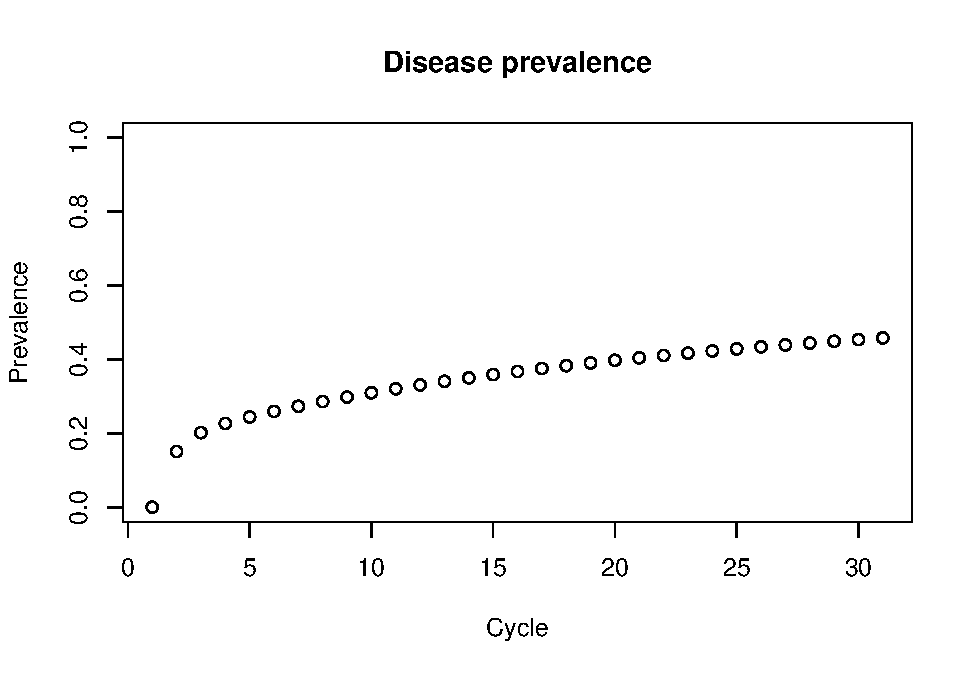
\includegraphics{microsim_Sick-Sicker_time_solutions_files/figure-latex/unnamed-chunk-12-1.pdf}

\begin{Shaded}
\begin{Highlighting}[]
\KeywordTok{plot}\NormalTok{(}\KeywordTok{density}\NormalTok{(outcomes_no_trt}\OperatorTok{$}\NormalTok{te), }\DataTypeTok{main =} \KeywordTok{paste}\NormalTok{(}\StringTok{"Total QALYs per person"}\NormalTok{), }\DataTypeTok{xlab =} \StringTok{"QALYs"}\NormalTok{)}
\end{Highlighting}
\end{Shaded}

\includegraphics{microsim_Sick-Sicker_time_solutions_files/figure-latex/unnamed-chunk-12-2.pdf}

\begin{Shaded}
\begin{Highlighting}[]
\KeywordTok{plot_m_TR}\NormalTok{(outcomes_no_trt}\OperatorTok{$}\NormalTok{m_M)  }\CommentTok{# health state trace}
\end{Highlighting}
\end{Shaded}

\includegraphics{microsim_Sick-Sicker_time_solutions_files/figure-latex/unnamed-chunk-12-3.pdf}

\begin{Shaded}
\begin{Highlighting}[]
\CommentTok{# Treatment}
\KeywordTok{plot}\NormalTok{(}\KeywordTok{density}\NormalTok{(outcomes_trt}\OperatorTok{$}\NormalTok{tc), }\DataTypeTok{main =} \KeywordTok{paste}\NormalTok{(}\StringTok{"Total cost per person"}\NormalTok{), }\DataTypeTok{xlab =} \StringTok{"Cost ($)"}\NormalTok{)}
\end{Highlighting}
\end{Shaded}

\includegraphics{microsim_Sick-Sicker_time_solutions_files/figure-latex/unnamed-chunk-12-4.pdf}

\begin{Shaded}
\begin{Highlighting}[]
\KeywordTok{plot}\NormalTok{(}\KeywordTok{density}\NormalTok{(outcomes_trt}\OperatorTok{$}\NormalTok{te), }\DataTypeTok{main =} \KeywordTok{paste}\NormalTok{(}\StringTok{"Total QALYs per person"}\NormalTok{), }\DataTypeTok{xlab =} \StringTok{"QALYs"}\NormalTok{)}
\end{Highlighting}
\end{Shaded}

\includegraphics{microsim_Sick-Sicker_time_solutions_files/figure-latex/unnamed-chunk-12-5.pdf}

\begin{Shaded}
\begin{Highlighting}[]
\KeywordTok{plot_m_TR}\NormalTok{(outcomes_trt}\OperatorTok{$}\NormalTok{m_M)     }\CommentTok{# health state trace}
\end{Highlighting}
\end{Shaded}

\includegraphics{microsim_Sick-Sicker_time_solutions_files/figure-latex/unnamed-chunk-12-6.pdf}

\hypertarget{cost-effectiveness-analysis}{%
\section{08 Cost-Effectiveness
Analysis}\label{cost-effectiveness-analysis}}

\begin{Shaded}
\begin{Highlighting}[]
\CommentTok{# store the mean costs of each strategy in a new variable C (vector of costs)}
\NormalTok{v_C <-}\StringTok{ }\KeywordTok{c}\NormalTok{(outcomes_no_trt}\OperatorTok{$}\NormalTok{tc_hat, outcomes_trt}\OperatorTok{$}\NormalTok{tc_hat)}
\CommentTok{# store the mean QALYs of each strategy in a new variable E (vector of effects)}
\NormalTok{v_E <-}\StringTok{ }\KeywordTok{c}\NormalTok{(outcomes_no_trt}\OperatorTok{$}\NormalTok{te_hat, outcomes_trt}\OperatorTok{$}\NormalTok{te_hat)}

\CommentTok{# use dampack to calculate the ICER}
\KeywordTok{calculate_icers}\NormalTok{(}\DataTypeTok{cost       =}\NormalTok{ v_C,}
                \DataTypeTok{effect     =}\NormalTok{ v_E,}
                \DataTypeTok{strategies =}\NormalTok{ v_names_str)}
\end{Highlighting}
\end{Shaded}

\begin{verbatim}
##       Strategy      Cost   Effect Inc_Cost Inc_Effect     ICER Status
## 1 no treatment  77752.46 16.19202       NA         NA       NA     ND
## 2    treatment 144839.47 16.76875 67087.01   0.576735 116322.1     ND
\end{verbatim}

\end{document}
